\documentclass{amsart}

\usepackage[utf8]{inputenc}
\usepackage[T2A]{fontenc}
\usepackage[english,russian]{babel}
\usepackage{amsthm,amsmath,amsfonts,amssymb}
\usepackage{fullpage}
\usepackage{eufrak}
\usepackage{bbm}

%%% Дополнительная работа с математикой
\usepackage{amsfonts,amssymb,amsthm,mathtools} % AMS
\usepackage{amsmath}
\usepackage{icomma}

%% Шрифты
\usepackage{euscript}	% Шрифт Евклид
\usepackage{mathrsfs}	% Красивый матшрифт

%% Свои команды
\DeclareMathOperator{\lb}{\mathop{lb}}	% логарифм по основанию 2
\DeclareMathOperator{\sgn}{\mathop{sgn}}	% сигнум
\renewcommand{\Im}{\mathop{\mathrm{Im}}\nolimits}	% мнимая часть
\renewcommand{\Re}{\mathop{\mathrm{Re}}\nolimits}	% вещественная часть
\renewcommand{\emptyset}{\varnothing}	% пустое множество
\renewcommand{\le}{\leqslant}	% отечественная версия "меньше или равно"
\renewcommand{\ge}{\geqslant}	% отечественная версия "больше или равно"
\renewcommand{\epsilon}{\varepsilon}	% стандартная "эпсилон"
\renewcommand{\phi}{\varphi}	% стандартная "фи"
\newcommand{\const}{\mathrm{const}}	% константа

%% Множества чисел
\DeclareMathOperator{\Natural}{\mathbb{N}}	% Натуральные числа
\DeclareMathOperator{\Integer}{\mathbb{Z}}	% Целые числа
\DeclareMathOperator{\Integerp}{\mathbb{Z}_{+}}	% Целые неотрицательные числа
\DeclareMathOperator{\Rational}{\mathbb{Q}}	% Рациональные числа
\DeclareMathOperator{\Real}{\mathbb{R}}	% Вещественные числа
\DeclareMathOperator{\Realp}{\mathbb{R}_{>0}}	% Вещественные положительные числа
\DeclareMathOperator{\Realn}{\mathbb{R}_{<0}}	% Вещественные отрицательные числа
\DeclareMathOperator{\Realnn}{\mathbb{R}_{\ge 0}}	% Вещественные неотрицательные числа
\DeclareMathOperator{\Realnp}{\mathbb{R}_{\le 0}}	% Вещественные неположительные числа
\DeclareMathOperator{\Complex}{\mathbb{C}}	% Комплексные числа

%% Заглавные греческие буквы
\DeclareMathOperator{\Alpha}{\mathrm{A}}	% Альфа
\DeclareMathOperator{\Beta}{\mathrm{B}}	% Вета
\DeclareMathOperator{\Epsilon}{\mathrm{E}}	% Эпсилон
\DeclareMathOperator{\Zeta}{\mathrm{Z}}	% Дзета
\DeclareMathOperator{\Eta}{\mathrm{H}}	% Эта
\DeclareMathOperator{\Iota}{\mathrm{I}}	% Йота
\DeclareMathOperator{\Kappa}{\mathrm{K}}	% Каппа
\DeclareMathOperator{\Mu}{\mathrm{M}}	% Мю
\DeclareMathOperator{\Nu}{\mathrm{N}}	% Ню
\DeclareMathOperator{\Omicron}{\mathrm{O}}	% Омикрон
\DeclareMathOperator{\Rho}{\mathrm{P}}	% Ро
\DeclareMathOperator{\Tau}{\mathrm{T}}	% Тау
\DeclareMathOperator{\Chi}{\mathrm{X}}	% Хи

%% Теория вероятностей
\renewcommand{\Prob}{\mathbb P}	% вероятность
\newcommand{\Expect}{\mathbb E}	% математическое ожидание
\renewcommand{\Variance}{\mathbb D}	% дисперсия
\newcommand{\Entropy}{\mathbb H}	% энтропия
\DeclareMathOperator{\cov}{\mathop{cov}}	% ковариация
\DeclareMathOperator{\supp}{\mathop{supp}}	% носитель
\DeclareMathOperator{\Skewness}{\mathop{Skew}}	% коэффициент асимметрии
\DeclareMathOperator{\Kurtosis}{\mathop{Kurt}}	% коэффициент эксцесса

%%% Статистический анализ
\newcommand*{\moment}[1]{\overline{#1}}	% выборочный момент
\DeclareMathOperator{\hskew}{\mathop{\widehat{Skew}}}	% выборочный коэффициент асимметрии
\DeclareMathOperator{\hkurt}{\mathop{\widehat{Kurt}}}	% выборочный коэффициент эксцесса
%% Однопараметрические распределения
\newcommand*{\chisq}[1]{\chi^2_{#1}}	% Распределение хи-квадрат
\newcommand*{\Stud}[1]{\mathcal{S}_{#1}}	% Распределение Стьюдента
\newcommand*{\Exp}[1]{\mathop{\mathrm{Exp}}(#1)}	% Показательное распределение
\newcommand*{\Bern}[1]{\mathop{\mathrm{Bern}}(#1)}	% Распределение Бернулли
\newcommand*{\Geom}[1]{\mathop{\mathrm{Geom}}(#1)}	% Геометрическое распределение
\newcommand*{\Pois}[1]{\mathop{\mathrm{Pois}}(#1)}	% Распределение Пуассона
%% Двухпараметрические распределения
\newcommand*{\FS}[2]{\mathcal{F}_{#1, #2}}	% Распределение Фишера-Снедекора
\newcommand*{\Norm}[2]{\mathcal{N}(#1, #2)}	% Нормальное распределение
\newcommand*{\Unif}[2]{\mathcal{U}(#1, #2)}	% Равномерное распределение
\newcommand*{\DE}[2]{\mathop{\mathrm{DE}}(#1, #2)}	% Распределение Лапласа
\newcommand*{\Cauchy}[2]{\mathop{\mathrm{C}}(#1, #2)}	% Распределение Коши
\newcommand*{\Binom}[2]{\mathop{\mathrm{Binom}}(#1, #2)}	% Биномиальное распределение
\newcommand*{\Betadist}[2]{\mathop{\mathrm{Beta}}(#1, #2)}	% Бета-распределение
\newcommand*{\Gammadist}[2]{\mathop{\mathrm{Gamma}}(#1, #2)}	% Гамма-распределение
%% Ажурные и готические буквы
\newcommand*{\Acl}{\mathcal{A}}	% A красивое
\newcommand*{\Ccl}{\mathcal{C}}	% C красивое
\newcommand*{\Fcl}{\mathcal{F}}	% F красивое
\newcommand*{\Icl}{\mathcal{I}}	% I красивое
\newcommand*{\Kcl}{\mathcal{K}}	% K красивое
\newcommand*{\Pcl}{\mathcal{P}}	% P красивое
\newcommand*{\Ycl}{\mathcal{Y}}	% Y красивое
\newcommand*{\Afr}{\mathfrak{A}}	% A готическое
\newcommand*{\Bfr}{\mathfrak{B}}	% B готическое
\newcommand*{\Ffr}{\mathfrak{F}}	% F готическое
\newcommand*{\Kfr}{\mathfrak{K}}	% K готическое
\newcommand*{\Xfr}{\mathfrak{X}}	% X готическое
%% Теория оценивания
\newcommand*{\ind}[1]{\mathbbm{1}_{\lbrace #1 \rbrace}}	% индикаторная функция
\newcommand*{\bias}[2]{\mathop{\mathrm{bias}}\nolimits_{#1}(#2)}	% смещение

%% Перенос знаков в формулах (по Львовскому)
\newcommand*{\hm}[1]{#1\nobreak\discretionary{}
	{\hbox{$\mathsurround=0pt #1$}}{}}

%%% Работа с картинками
\usepackage{graphicx,xcolor}	% Для вставки рисунков
\graphicspath{{images/}{images2/}}	% папки с картинками
\setlength\fboxsep{3pt}	% Отступ рамки \fbox{} от рисунка
\setlength\fboxrule{1pt}	% Толщина линий рамки \fbox{}
\usepackage{wrapfig}	% Обтекание рисунков и таблиц текстом
\RequirePackage{caption}
\DeclareCaptionLabelSeparator{defffis}{ "--- }
\captionsetup{justification=centering,labelsep=defffis}
\usepackage{float}
\usepackage{tikz}
\usepackage{pgfplots}
\pgfplotsset{compat=newest}
\usetikzlibrary{patterns}
\usetikzlibrary{calc}

%%% Работа с таблицами
\usepackage{array,tabularx,tabulary,booktabs}	% Дополнительная работа с таблицами
\usepackage{longtable}	% Длинные таблицы
\usepackage{multirow}	% Слияние строк в таблице
\usepackage{makecell}
\usepackage{multicol}


\renewcommand{\qedsymbol}{}

\newtheorem{problem}{Задание}

\begin{document}
	\newcommand{\problemset}[1]{
		\begin{center}
			\Large #1
		\end{center}
	}

	\begin{tabbing}
	\hspace{11cm} \= Студент: \= Майоров Артемий \\	% не забудьте исправить, студент Вы или студентка :)
																									% (а то некоторые забывают)
	\> Группа: \> 2375 \\	% Здесь меняете № группы
	\> Вариант: \> 14 \\		% А здесь меняете № варианта
	\> Дата: \> \today		% А вот здесь ничего не меняем!!!
\end{tabbing}
\hrule
\vspace{1cm}	% файл с заголовком
	\problemset{Теория вероятностей и математическая статистика}
\problemset{Индивидуальное домашнее задание №3}

% Команда ниже задает "название" или слово, которое будет
% отображаться вместо proof или "доказательство"
% поскольку у нас в ИДЗ задачи - то нужно слово "Решение"
\renewcommand*{\proofname}{Решение}

Случайный вектор $(\xi,\eta)$ имеет равномерное распределение в области $D$:
\[
D = \{(x,y)\text{ }|\text{ }4x + 4y \le 12, x \ge -2, y \ge 1\}
\]
$\zeta = 2\xi^3 - 3$, $\nu = \lfloor 5\eta\rfloor$, $\mu = 8\xi + 8\eta$

%%%%%%%%%%%%%% ЗАДАНИЕ №1 %%%%%%%%%%%%%%
%% Условие задания №1
\begin{problem}
Найти $p_{\xi,\eta}(x,y)$, функции и плотности распределения компонент. Построить графики функций распределений $F_{\xi}(x)$ и $F_{\eta}(y)$. Будут ли компоненты независимыми?
\end{problem}

%% Решение задания №1
\begin{proof}
Равномерное распределение \Rightarrow
\[
p_{\xi,\eta}(x,y) = \begin{cases}
    C, & (x,y) \in D\\
    0, & \text{в отс. сл.}
    \end{cases}
\]\\
\begin{figure}[H]
    \centering
    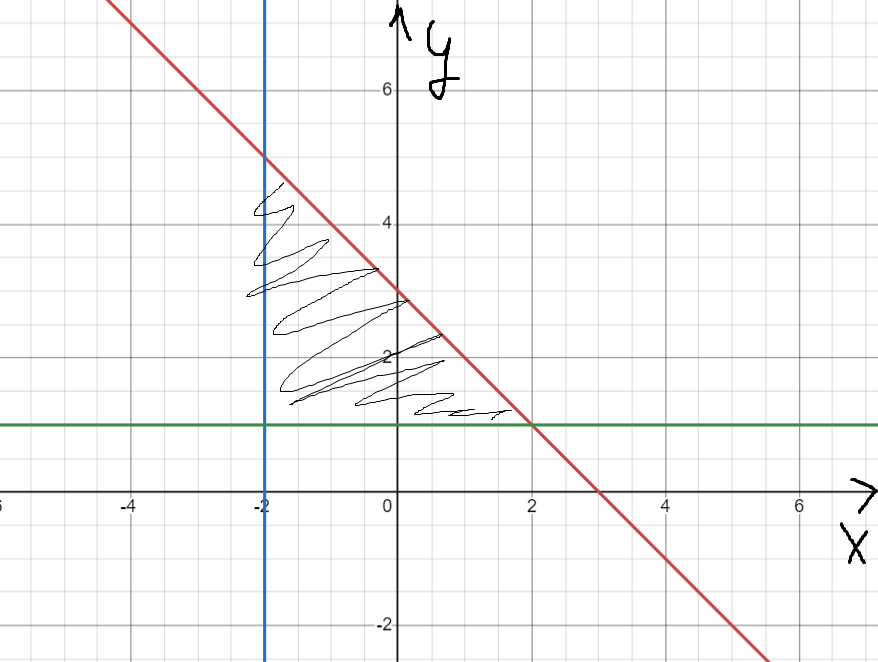
\includegraphics[width=0.5\linewidth]{3idz_0png.png}
    \caption{}
    \label{fig:enter-label}
\end{figure}
$ \iint_{\Real^2}p_{\xi,\eta}(x,y)dxdy = 1$:
\[
\iint_{\Real^2}p_{\xi,\eta}(x,y)dxdy = \iint_{D}p_{\xi,\eta}(x,y)dxdy = \int_{-2}^{2}dx\int_{1}^{3-x}Cdy = 1 \Rightarrow C = \frac{1}{8}
\]

\[
p_{\xi,\eta}(x,y) = \begin{cases}
    \frac{1}{8}, & (x,y) \in D\\
    0, & \text{в отс. сл.}
    \end{cases}
\]
Плотности распределений.\\
Для компоненты $\xi$:
\begin{gather*}
\int_{\Real}p_{\xi,\eta}(x,y)dy = \int_{1}^{3-x}\frac{1}{8}dy = \frac{2-x}{8}\\
p_{\xi}(x) = \begin{cases}
    \frac{2-x}{8}, & x \in [-2;2]\\
    0, & \text{в отс. сл.}
    \end{cases}
\end{gather*}
Для компоненты $\eta$:
\begin{gather*}
\int_{\Real}p_{\xi,\eta}(x,y)dx = \int_{-2}^{3-y}\frac{1}{8}dx = \frac{5-y}{8}\\
p_{\eta}(x) = \begin{cases}
    \frac{5-y}{8}, & y \in [1;5]\\
    0, & \text{в отс. сл.}
    \end{cases}
\end{gather*}
Проверка на независимость: $p_{\xi,\eta}(x,y) = p_{\xi}(x)\cdot p_{\eta}(y)$ во всех точках D.
\[
\frac{1}{8} = \frac{2-x}{8}\cdot\frac{5-y}{8}\\
\]
Рассмотрим точку (0,0):
\[
\frac{1}{8} = \frac{2-x}{8}\cdot\frac{5-y}{8} = \frac{10}{64} - \text{неверно}\Rightarrow\text{зависимы}
\]

\[
F_{\xi}(x) = \int\limits_{-\infty}^{x}p_{\xi}(t)dt = \begin{cases}
    0, & x\in (-\infty;-2]\\
    \frac{-x^2 + 4x + 12}{16}, & x\in (-2; 2]\\
    1, & x\in (2;\infty)
\end{cases}
\]
\[
F_{\eta}(y) = \int\limits_{-\infty}^{y}p_{\eta}(t)dt = \begin{cases}
    0, & y\in (-\infty;1]\\
    \frac{-y^2 + 10y - 9}{16}, & y\in (1; 5]\\
    1, & y\in (5;\infty)
\end{cases}
\]

\begin{figure}[H]
    \centering
    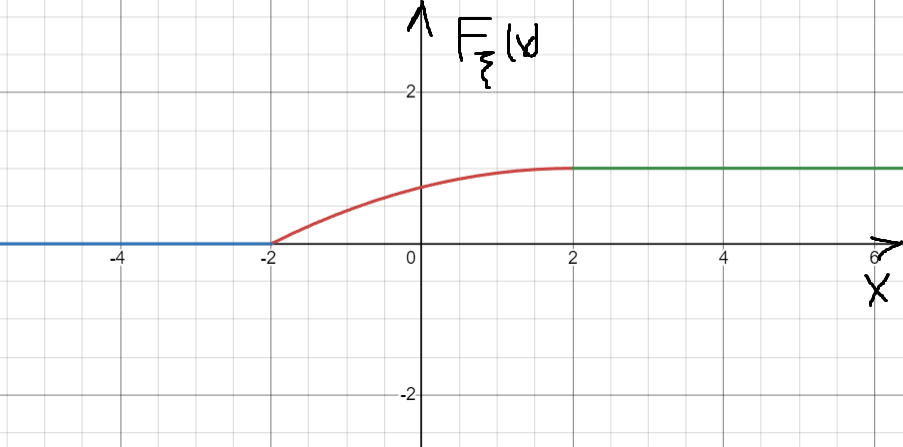
\includegraphics[width=0.5\linewidth]{3idz_1png.png}
    \caption{}
    \label{fig:enter-label}
\end{figure}
\\

\begin{figure}[H]
    \centering
    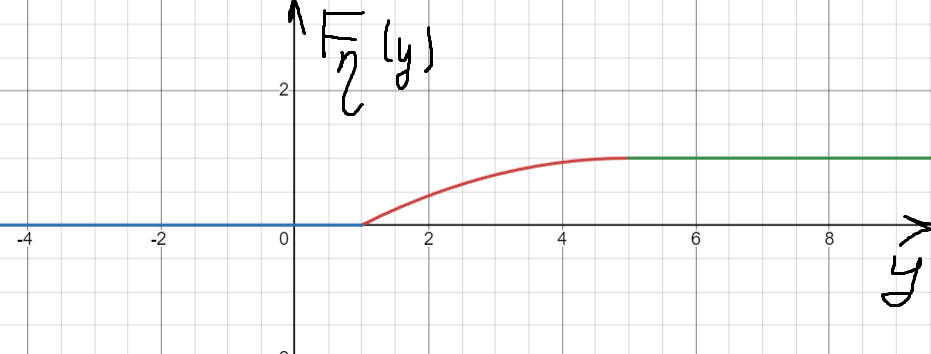
\includegraphics[width=0.5\linewidth]{3idz_2png.png}
    \caption{}
    \label{fig:enter-label}
\end{figure}
\end{proof}

%%%%%%%%%%%%%% ЗАДАНИЕ №2 %%%%%%%%%%%%%%
%% Условие задания №2
\begin{problem}
Найти распределения случайных величин $\zeta$ и $\nu$. Вычислить $\Expect\zeta$, $\Variance\zeta$, $\Expect\nu$ и $\Variance\nu$. Построить графики функций распределений $F_{\zeta}(z)$ и $F_{\nu}(n)$.
\end{problem}

%% Решение задания №2
\begin{proof}
$\zeta = 2\xi^3 - 3$. $\supp\xi = [-2;2]$, $\supp\zeta = [-19;13]$. $g(\xi) = 2\xi^3 - 3$ и $g(\xi)$ монотонно возрастает на $\supp\xi$. Тогда:
\begin{gather*}
g^{-1}(z) = \sqrt[3]{\frac{z + 3}{2}}\\
(g^{-1}(z))' = \frac{\sqrt[3]{4}}{6\sqrt[3]{(z + 3)^2}}\\
\end{gather*}
Воспользуемся формулой для нахождения плотности распределения:\\
$p_{\zeta}(z) = \frac{1}{|(g^{-1}(z))'|} \cdot p_\xi(g^{-1}(z))$\\
\[
p_{\zeta}(z) = \begin{cases}
    \frac{\sqrt[3]{4}}{6\sqrt[3]{(z + 3)^2}}\cdot \frac{2 - \sqrt[3]{\frac{z+3}{2}}}{8}, & z \in [-19;13]\\
    0, & \text{в отс. сл.}
    \end{cases}
\]
Функция распределения (график на рис. 3):
\[
F_{\zeta}(z) = \int\limits_{-\infty}^{z}p_{\zeta}(t)dt = \begin{cases}
    0, & z\in (-\infty;-19]\\
    -\dfrac{\left(z+3\right)^\frac{2}{3}-8\sqrt[3]{z+3}-2^\frac{13}{3}-2^\frac{8}{3}}{4^\frac{8}{3}}, & z\in (-19; 13]\\
    1, & z\in (13;\infty)
\end{cases}
\]

\begin{figure}[H]
    \centering
    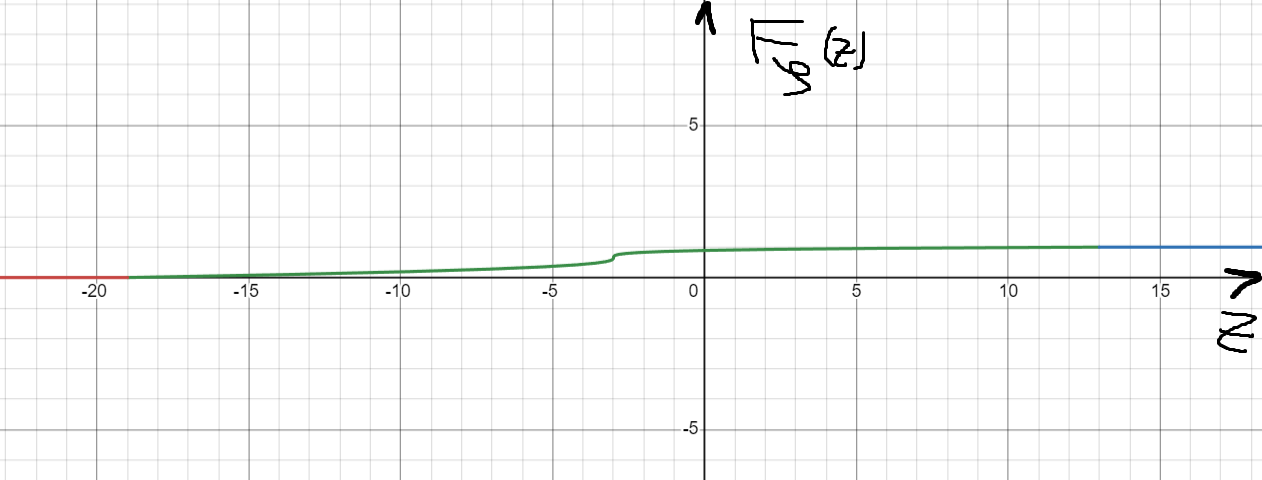
\includegraphics[width=0.5\linewidth]{3idz_3.png}
    \caption{}
    \label{fig:enter-label}
\end{figure}
\\
\begin{gather*}
    \Expect\zeta = \int_{-\infty}^{\infty}z\cdot p_{\zeta}(z)dz = \int_{-19}^{13}z\cdot p_{\zeta}(z)dz = -6.2\\
    \Expect\zeta^2 = \int_{-\infty}^{\infty}z^2\cdot p_{\zeta}(z)dz = \int_{-19}^{13}z^2\cdot p_{\zeta}(z)dz = 64.7714\\
    \Variance\zeta = \Expect\zeta^2 - \left(\Expect\zeta\right)^2 = 26.3314
\end{gather*}
\\
$\nu = \lfloor5\eta\rfloor$. $\supp\eta = [1;5]$, $\supp\nu = [5;24]$.
$
\Prob(\nu = k) = \Prob(\eta\in[k/5; (k + 1)/5)) = \int_{\frac{k}{5}}^{\frac{k + 1}{5}}\frac{5-y}{8}dy = \frac{49-2k}{400}
$\\
Для построения графика функции распределения будем подставлять целочисленные значения $\nu$:

\begin{table}[H]
    \centering
    \begin{tabular}{|c|c|c|c|c|c|c|c|c|c|c|c|c|c|c|c|c|c|c|c|c|c|}
    \hline
        $\nu$ & 5 & 6 & 7 & 8 & 9 & 10 & 11 & 12 & 13 & 14 & 15 & 16 & 17\\
    \hline
        $p_i$& 0.0975 & 0.19 & 0.2775 & 0.36 & 0.4375 & 0.51 & 0.5775 & 0.64 & 0.6975 & 0.75 & 0.7975 & 0.84 & 0.8775\\
    \hline
        $\nu$& 18 & 19 & 20 & 21 & 22 & 23 & 24 & $\sum$\\
    \hline
        $p_i$& 0.91 & 0.9375 & 0.96 & 0.9775 & 0.99 & 0.9975 & 1 & 1\\
    \hline
    \end{tabular}
\end{table}

\[
F_{\nu}(n) = \begin{cases}
    0, & n\in (-\infty;5]\\
    0.0975, & n\in (5;6]\\
    0.19, & n\in (6;7]\\
    0.2775, & n\in (7;8]\\
   0.36, & n\in (8;9]\\
     0.4375, & n\in (9;10]\\
     0.51, & n\in (10;11]\\
    0.5775, & n\in (11;12]\\
    0.64 , & n\in (12;13]\\
    0.6975, & n\in (13;14]\\
    0.75, & n\in (14;15]\\
    0.7975, & n\in (15;16]\\
   0.84, & n\in (16;17]\\
    0.8775, & n\in (17;18]\\
   0.91, & n\in (18;19]\\
    0.9375, & n\in (19;20]\\
    0.91, & n\in (20;21]\\
    0.96, & n\in (21;22]\\
    0.99, & n\in (22;23]\\
     0.9975, & n\in (23;24]\\
    1, & n\in (24;25]\\
    1, & n\in (25;\infty)
\end{cases}
\]

\begin{figure}[H]
    \centering
    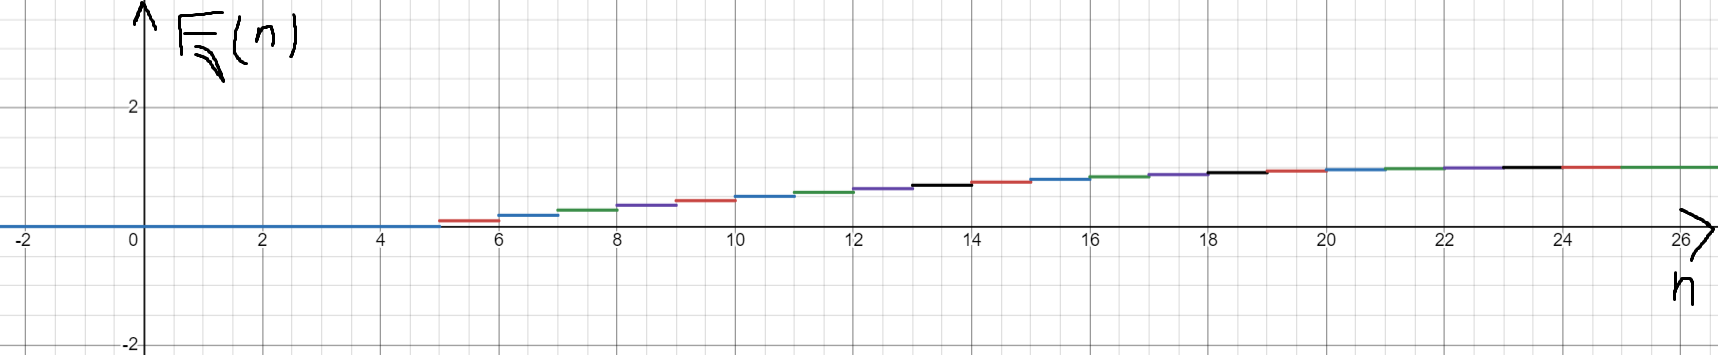
\includegraphics[width=0.5\linewidth]{3idz_4png.png}
    \caption{}
    \label{fig:enter-label}
\end{figure}

\begin{gather*}
    \Expect\nu = \sum_{i: p_i > 0}a_ip_i = 11,175\\
    \Expect\nu^2 = \sum_{i: p_i > 0}a_i^2p_i = 147,075\\
    \Variance\nu = \Expect\nu^2 - \left(\Expect\nu\right)^2 = 22,1944
\end{gather*}
\end{proof}

%%%%%%%%%%%%%% ЗАДАНИЕ №3 %%%%%%%%%%%%%%
%% Условие задания №3
\begin{problem}
Вычислить вектор математических ожиданий, построить ковариационную и кореляционную матрицы для вектора $(\xi,\eta)$. Найти условное распределение $\xi$ при условии $\eta$. Вычислить $\Expect(\xi | \eta)$ и $\Variance(\xi | \eta)$.
\end{problem}

%% Решение задания №3
\begin{proof}
Мат.ожидание и дисперсия для $\xi$:
\begin{gather*}
    \Expect\xi = \int_{-\infty}^{\infty}x\cdot p_{\xi}(x)dx = \int_{-2}^{2}x\cdot\frac{2-x}{8}dx = -\frac{2}{3}\\
    \Expect\xi^2 = \int_{-\infty}^{\infty}x^2\cdot p_{\xi}(x)dx = \int_{-2}^{2}x^2\cdot\frac{2-x}{8}dx = \frac{4}{3}\\
    \Variance\xi = \Expect\xi^2 - \left(\Expect\xi\right)^2 = \frac{4}{3} - \frac{4}{9} = \frac{8}{9}
\end{gather*}
Мат.ожидание и дисперсия для $\eta$:
\begin{gather*}
    \Expect\eta = \int_{-\infty}^{\infty}y\cdot p_{\eta}(y)dy = \int_{1}^{5}y\cdot\frac{5-y}{8}dy = \frac{7}{3}\\
    \Expect\eta^2 = \int_{-\infty}^{\infty}y^2\cdot p_{\eta}(y)dy = \int_{1}^{5}y^2\cdot\frac{5-y}{8}dy = \frac{19}{3}\\
    \Variance\eta = \Expect\eta^2 - \left(\Expect\eta\right)^2 = \frac{19}{3} - \frac{49}{9} = \frac{8}{9}
\end{gather*}
Вектор мат.ожиданий:\\
\[
\Expect\begin{pmatrix} \xi \\ \eta \end{pmatrix} = \begin{pmatrix} -2/3 \\ 7/3 \end{pmatrix}
\]
Посчитаем ковариацию и корреляцию $\xi$ и $\eta$:
\begin{gather*}
\Expect\xi,\eta = \iint_{\Real^2}xy\cdot p_{\xi,\eta}(x,y)dxdy = \int_{-2}^{2}dx\int_{1}^{3-x}\frac{1}{8}xydy = -2\\
\cov(\xi, \eta) = \Expect\xi\eta - \Expect\xi\cdot\Expect\eta = -\frac{4}{9}\\
\rho(\xi,\eta) = \frac{\cov(\xi,\eta)}{\sqrt{\Variance\xi}\sqrt{\Variance\eta}} = -\frac{1}{2}
\end{gather*}
Матрицы:
\[
\sum = \begin{pmatrix}
\frac{8}{9} & -\frac{4}{9} \\
-\frac{4}{9} & \frac{8}{9}
\end{pmatrix}
\]
\[
R = \begin{pmatrix}
1 & -\frac{1}{2} \\
-\frac{1}{2} & 1
\end{pmatrix}
\]
Найдем условное распределение $\xi$ при условии $\eta$:
\begin{gather*}
    p_{\xi|\eta=y_0} = \frac{p_{\xi,\eta}(x,y_0)}{p_{\eta}(y_0)}\\
     p_{\xi|\eta=y_0} = \begin{cases}
        \frac{1}{5-y_0}, & x\in [-2;3-y_0]\\
        0, & \text{в отс. сл.}
    \end{cases} \\
     p_{\xi|\eta} = \begin{cases}
        \frac{1}{5-\eta}, & x\in [-2;3-\eta]\\
        0, & \text{в отс. сл.}
    \end{cases}
\end{gather*}
Условное мат.ожидание и условная дисперсия:
\begin{gather*}
    \Expect(\xi|\eta) = \int_{-\infty}^{\infty}x\cdot p_{\xi|\eta}(x)dx = \int_{-2}^{3-\eta}x\cdot p_{\xi|\eta}(x)dx = -\dfrac{\eta-1}{2}\\
    \Expect(\xi^2|\eta) = \int_{-\infty}^{\infty}x^2\cdot p_{\xi|\eta}(x)dx = \int_{-2}^{3-\eta}x^2\cdot p_{\xi|\eta}(x)dx =-\dfrac{\eta^2-4\eta+7}{3}\\
    \Variance(\xi|\eta) = \Expect(\xi^2|\eta) - \left(\Expect(\xi|\eta)\right)^2 = \frac{(\eta-5)^2}{12}
\end{gather*}
Проверим свойство $\Expect(\Expect(\xi|\eta)) = \Expect\xi$:
\[
\Expect(\Expect(\xi|\eta)) = \Expect\left(\frac{1-\eta}{2}\right) = \Expect\left(\frac{1}{2}\right) - \frac{1}{2}\Expect\left(\eta\right) = \frac{1}{2}\left(1 - \frac{7}{3}\right) = -\frac{2}{3} = \Expect\xi - \text{верно}
\]
Проверим свойство $\Expect(\Variance(\xi|\eta)) + \Variance(\Expect(\xi|\eta)) = \Variance\xi$:
\[
\Expect(\Variance(\xi|\eta)) + \Variance(\Expect(\xi|\eta)) = \Expect\left(\frac{(\eta-5)^2}{12}\right) + \Variance\left(\frac{1-\eta}{2}\right) = \frac{2}{3} + \frac{2}{9} = \frac{8}{9} = \Variance\xi - \text{верно}
\]\\
Следовательно мат. ожидания и дисперсии найдены верно.\\
\end{proof}

%%%%%%%%%%%%%% ЗАДАНИЕ №4 %%%%%%%%%%%%%%
%% Условие задания №4
\begin{problem}
Найти распределение $\mu$. Вычислить $\Expect\mu$ и $\Variance\mu$. Построить график функции распределения $F_{\mu}(m)$.
\end{problem}

%% Решение задания №4
\begin{proof}
\begin{figure}[H]
    \centering
    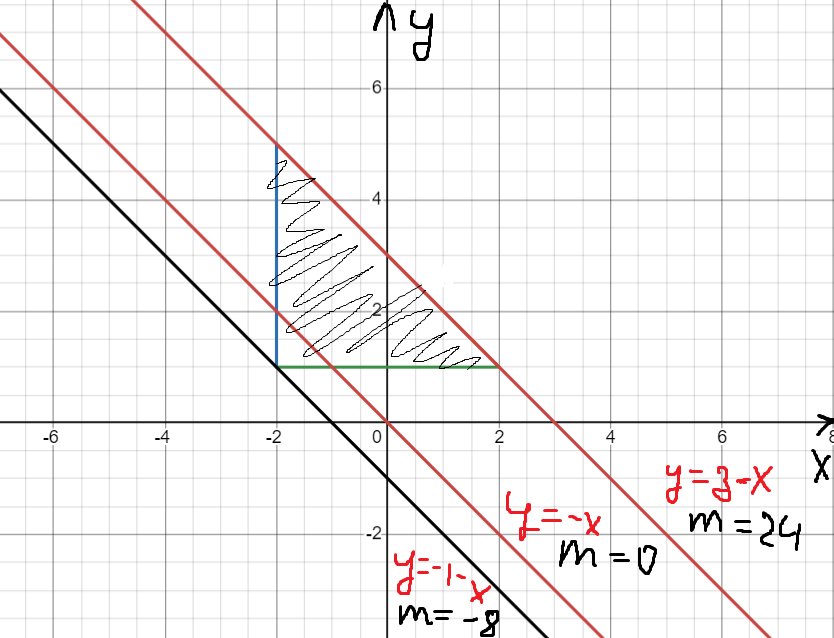
\includegraphics[width=0.5\linewidth]{3idz_5png.png}
    \caption{}
    \label{fig:enter-label}
\end{figure}
$\mu = 8\xi + 8\eta$. $F_{\mu}(m) = \Prob(8\xi + 8\eta\le m)$.\\
$m = 8x + 8y \Rightarrow y = \frac{m-8x}{8} \Rightarrow x = \frac{m-8y}{8}$\\
$\begin{cases}
\supp \xi = [-2;2]\\
\supp \eta = [1;5]
\end{cases} \Rightarrow \supp \mu = [-8;24]$\\
$F_{\mu}(m) = \int_{D}\int p_{\xi, \eta}(x, y)dxdy = \int_{-2}^{\frac{m-8}{8}}dx \int_{1}^{\frac{m-8x}{8}}\frac{1}{8}dy = \frac{1}{8}\int_{-2}^{\frac{m-8}{8}}\frac{m-8x-8}{8}dx = \frac{1}{8}\left(\frac{m-8}{8}\cdot \frac{m+8}{8} - \frac{(m-8)^{2} - 256}{128}\right) = \frac{m^2 + 16m + 64}{1024}$\\
$\\
F_{\mu}(m) = \begin{cases}
    0, & m\in (-\infty;-8]\\
    \frac{m^2 + 16m + 64}{1024}& m\in (-8; 24]\\
    1, & m\in (24; \infty)
\end{cases}
$\\

\begin{figure}[H]
    \centering
    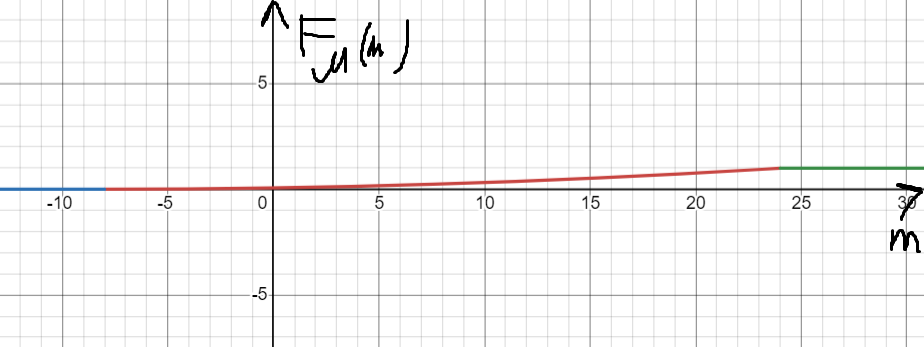
\includegraphics[width=0.5\linewidth]{3idz_6png.png}
    \caption{}
    \label{fig:enter-label}
\end{figure}
\end{proof}
\\
Находим плотность:
\\
$
p_{\mu}(m) = (F_{\mu}(m))' = \begin{cases}
    \dfrac{m+8}{512}& m\in [-8; 24]\\
    0, & \text{в отс. сл.}
\end{cases}
$\\
\\Мат.ожидание и дисперсия:\\
$
    \Expect\mu = \int_{-\infty}^{\infty}m\cdot p_{\mu}(m)dm = \int_{-8}^{24}m\cdot \dfrac{m+8}{512}dm = \dfrac{40}{3}\\
    \Expect\mu^2 = \int_{-\infty}^{\infty}m^2\cdot p_{\mu}(m)dm = \int_{-8}^{24}m^2\cdot \dfrac{m+8}{512}dm = \dfrac{704}{3}\\
    \Variance\mu = \Expect\mu^2 - \left(\Expect\mu\right)^2 = \frac{704}{3} - \frac{1600}{9} = \frac{512}{9}\\
$
	% файл с решениями
\end{document}